\section{Product perspective}
\label{sec:product_perspective}%

\subsection{Class Diagrams}
\label{subsec:class_diagrams}%
The diagram below represents and describes the classes involved in the system, their basic functionalities, attributes,
and the relationships between them.
Some suggestions for a further expansion and deepening of the diagram could be to evaluate the use of a decorator
pattern to implement the ``Fee'' class;
also, the use of a status pattern can be evaluated, in order to set the state of a charging point (free, booked, occupied, broken) in a more versatile way.
Furthermore, another suggestion could be to adopt the factory pattern to implement the ``plug'' interface.
\begin{figure}[H]
    \begin{center}
        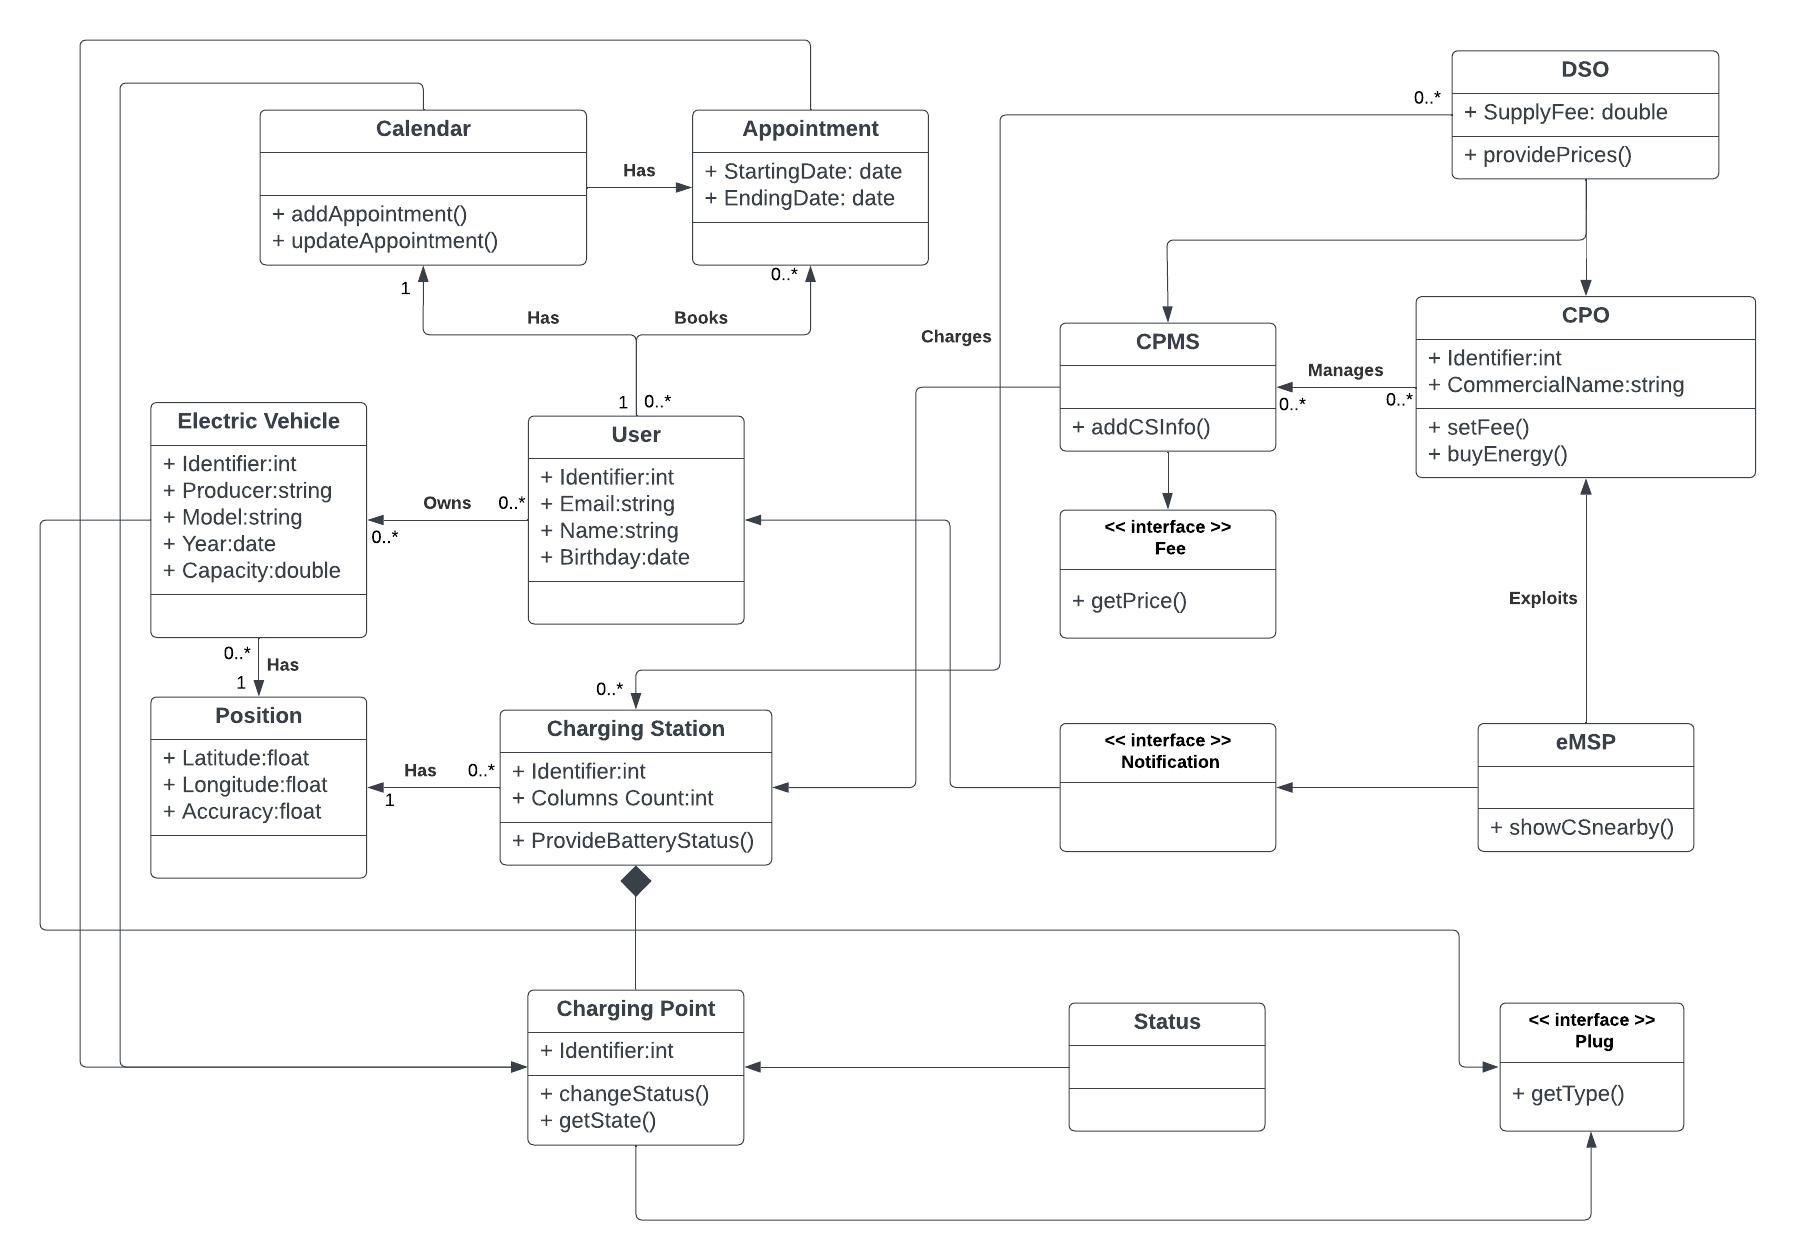
\includegraphics[width=0.9\linewidth]{ClassDiagrams/Class_Diagram_-_noPatterns}
        \caption{A simplified Class Diagram}
        \label{fig:class_diagram}%
    \end{center}
\end{figure}

\subsection{State Diagrams}
\label{subsec:state_diagrams}%

\paragraph{The EVD gets position and characteristics of charging stations at a certain location.}
EVD Andrew is going to use his car to go to the university for the Software Engineering 2 exam, but his EV is out of battery.
So, he needs to decide where to charge his vehicle.
To do that, he opens the \verb|eMALL| application and enters the map section.
At first, he sees if there is any charging station around him, but unfortunately at his current position,
there is only one charging station, which is shown as in maintenance.
So, he decides to see where to charge his EV nearby the university, inserting Milan in the location search bar.
From the huge amount of charging stations, he decides to choose the cheapest one.
He selects a charging station and gets its additional information.
He goes on searching other stations until he finds the best one for him.
At this point, the navigation process ends.

Below is presented a state diagram summarizing the flow of activities done in the charging stations navigation process:
\begin{figure}[H]
    \begin{center}
        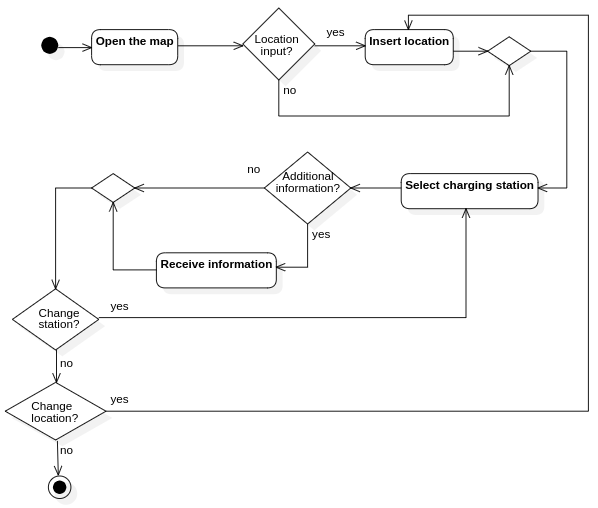
\includegraphics[width=0.8\linewidth]{StateDiagrams/get_charging_stations_location_state_diagram}
        \caption{Get locations of charging stations state diagram}
        \label{fig:locations_sd}%
    \end{center}
\end{figure}

\paragraph{EVD books a charge at a specified charging station at a certain timeframe.}
Andrew needs to book a charge for his EV\@.
He selects a charging station on the map and enters the booking section.
Unfortunately, the charging station cannot offer a reservation to him because no spots are available.
So, he searches for another one until he finds it.
Andrew has to decide in which timeframe he wants the charging point to be reserved.
So, he checks the availability schedule of the charging station and books a slot for its charge.
The system asks to pay a deposit to the EVD, which proceed to pay.
Finally, the EVD receives an e-mail with all the information that confirms the reservation.

It is shown a state diagram that summaries the activities in the booking process:
\begin{figure}[H]
    \begin{center}
        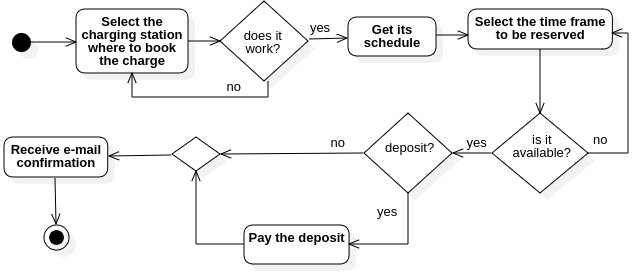
\includegraphics[width=0.9\linewidth]{StateDiagrams/book_a_charge_state_diagram}
        \caption{Book a charge state diagram}
        \label{fig:booking_sd}%
    \end{center}
\end{figure}

\paragraph{CPO adds charging points in its CPMS.}
\verb|SOLARIS| is the new company of the successful businessman Hugh Peter.
They decided to trust the \verb|eMALL| project, entrusting them with the responsibility of managing their IT infrastructure.
After logging in, they start inserting new charging points owned by them and distributed throughout the territory.
The first thing they are asked to select is the charging station to which the new spot belongs.
So, they insert all the requested information (serial number, location, connectors, power, etc.).
After they confirm and submit what they inserted, they iterate the process until they have inserted all the charging points.
It is shown a state diagram to summaries the activities in the charging points insertion process:
\begin{figure}[H]
    \begin{center}
        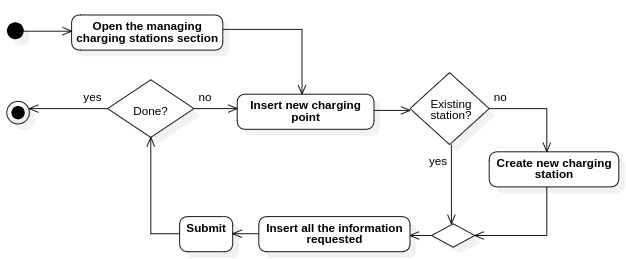
\includegraphics[width=0.9\linewidth]{StateDiagrams/insert_charging_points_state_diagram}
        \caption{Insert charging points state diagram}
        \label{fig:insert_charging_points_sd}%
    \end{center}
\end{figure}

\subsection{Scenarios}
\label{subsec:scenarios}%

\paragraph{Unregistered EVD creates an account.}
Mr. Oak has his EV and is looking for an application that offers the chance to charge his vehicle and smartly plan a
charging process depending on the battery status and his daily schedule.
Fortunately, he finds out \verb|eMALL|\@.
So, he immediately proceeds to create an account.
At first, he opens the application and goes to the ``sign up'' section.
The system asks to Mr. Oak if "he/she's a boy or a girl", in addition to personal information such as first and second name, birthday, living address, e-mail address, password, and telephone number, which he inserts immediately.
He receives an e-mail with a 6-digit code to be inserted in the new window shown by the \verb|eMALL| system to confirm his e-mail address.
After accepting the terms \& conditions and submitting all the inserted information, the system creates his account,
and he can begin using the application.

\paragraph{The EVD charges his/her EV.}
After booking a charge, Michael Scarn goes to the charging station at the chosen hour.
After turning off the EV, he opens the \verb|eMALL| application and enters the charge section.
From the set of close charging points, he selects which one has the serial number he received by \verb|eMALL| by e-mail
when he booked the charge.
So, he asks to charge the EV at that charging point.
After verifying that the EVD can be charged at that charging point, the application notifies to the user that the
connectors are now unlocked and ready to be used.\@
While the EV is in charge, the system notifies the EVD of the current status of the charging process.
When the process ends, he unplugs the connector, pays through the \verb|eMALL| application, and gets back in his car.

\paragraph{The EVD inserts a new activity in its calendar and receives a suggestion for a charging process.}
Jimothy inserts a new activity in his calendar, specifying the hour and destination of the event.
After doing that, he receives a notification that shows the EVD where and when to charge his vehicle.
The system creates suggestions to minimize the cost and the time lost at the charging station.
It also considers special offers activated by the CPOs registered in the eMALL system.
So, Joe accepts the received proposal and confirms the book of the listed charging points, making the needed payments.

\paragraph{The EVD receives a notification about a new special offer activated by a CPO}
Joe receives a notification about a new special offer activated by the CPO \verb|SOLARIS|.
So, he opens the promotion page, reads what it is about, and gets the discount code of the offer.
It consists of a 20\% discount for all the EVDs that are under 25.
Considering that he has to charge his EV, he decides to book a charging session at a charging station owned by the CPO \verb|SOLARIS|.
After selecting the timeframe and verifying its availability, he inserts the discount code SARTORIUS\@.


\section{Product functions}
\label{sec:product_functions}%
\textbf{The EVD books a charging session} \\
The main functionality of \verb|eMALL| is to book charge sessions in different charging stations for the EVD\@.
In particular, the system shows charging stations to the EVD and waits for him to select where he wants to book a charging session.

When \verb|eMALL| retrieves information about the charging stations available in the local area, it also retrieves all the extra info about the available plugs and power supplies.

The system has to control if the charging station is currently unavailable, and if it is not, it gets the station's schedule.
The EVD has to choose a timeframe between the ones available to book a charge session.
\verb|eMALL| also queries the charging station to know if the station has or not a mandatory deposit to pay to end the booking process.
If the station does not have a deposit policy, then \verb|eMALL| finishes the booking process by sending an informative email to the EVD that resumes all the booking info.

In the email, \verb|eMALL| also specifies the serial number associated with the charging point of the charging station where the EVD has to charge his EV\@.

\textbf{The EVD receives charging alerts about where to charge his EV} \\
\verb|eMALL| offers smart functions about when the EVD might book a charge for his EV\@.
Hence, when an EVD inserts a new activity in his calendar, \verb|eMALL| computes the best route to reach the destination through an external navigator API\@.
\verb|eMALL| also checks the battery status of the EV, so it notifies the best itinerary for the EVD\@.
If the battery state doesn't allow the EVD to reach the destination, then \verb|eMALL| shows him the best route with the charging stations available along the road.

\verb|eMALL| tries to minimize the costs.
Hence, starting from the current battery status, the system computes the maximum kilometers an EV can travel before running out of battery.
If the EV can reach the destination, \verb|eMALL| marks the route returned by the API as preferred.
On the other hand, \verb|eMALL| finds charging stations along the road and selects the one with the minimum costs because it knows the details about the EV, for instance, the plug type.
The best charging station found is shown to the EVD, allowing him to decide whether to start a booking process.

If the EVD doesn't accept \verb|eMALL| solution, he can book another charging station along the road and start, as well, a booking process.

\textbf{The CPO manages its charging stations} \\
A CPO should be able to manage its charging stations and relative charging points.
In general, a CPO might have new charging stations to register in \verb|eMALL|, and, as well, it might have charging points too.
The system allows the CPO to register charging stations, by entering all the info about them, for instance, the position on the map and the number of charging points available.
Furthermore, the system allows the registration of also charging points by inserting info like the available plugs and the power supply of the charging process.

Just like the CPO inserts new information about its product, it can also delete charging points or charging stations from \verb|eMALL|\@.

The system also shows CPOs charging stations and relative charging points on the map.
This functionality is necessary because they might break down, so the CPO has to change their availability status (offline, under maintenance, online).


\section{User characteristics}
\label{sec:user_characteristics}%
The actors listed below are considered in the eMALL system
\begin{itemize}
    \item \textbf{CPO:} owns one or more charging stations, and manages bookings and promotions about its charging points.
    He buys energy from DSOs, based on prices and needs.
    CPOs has their own IT system.
    \item \textbf{Unregistered EV Driver:} anybody who owns an electric vehicle, but isn’t registered in the eMALL system.
    Before accessing its benefits, it needs to get an account.
    \item \textbf{Registered EV Driver:} an electric vehicle owner who already joined the eMALL system, and access its benefits.
    He’s identified with a unique ID, and can own one or more vehicles with different specifics.
    They can check prices and position of charging points, in addition to receiving notifications about promotions reserved to them.
\end{itemize}


\section{Assumptions, dependencies and constraints}
\label{sec:assumptions_dependencies_and_constraints}%
\newcounter{da}
\setcounter{da}{1}
\newcommand{\cda}{\theda\stepcounter{da}}
\begin{center}
    \begin{longtable}{ |l|p{0.9\linewidth}| }
        \hline
        \textbf{ID} & \textbf{Description}                                                                                     \\
        \hline
        DA\cda      & Each user has needed competences to use the \verb|eMALL| system.                                         \\
        \hline
        DA\cda      & Both the users EVDs and CPOs have an e-mail.                                                             \\
        \hline
        DA\cda      & The EVD has a payment method.                                                                            \\
        \hline
        DA\cda      & The EVD uses a device with internet connectivity.                                                        \\
        \hline
        DA\cda      & The EVD uses a device with GPS module for navigation and localization.                                   \\
        \hline
        DA\cda      & There is a specific compatibility between EV's plug and connectors offered by charging points.           \\
        \hline
        DA\cda      & Charging points have their own software.                                                                 \\
        \hline
        DA\cda      & Communication between the \verb|eMALL| system and the charging points happens through the OCPP protocol. \\
        \hline
        DA\cda      & The \verb|eMALL| system communicates with EV brands API to get vehicles' specification.                  \\
        \hline
        DA\cda      & The \verb|eMALL| system communicates with DSOs through their APIs.                                       \\
        \hline
        DA\cda      & The \verb|eMALL| system communicates with third-party payment services to manage the payments.           \\
        \hline
        \caption{Domain assumptions.}
        \label{tab:domainassmptn_tab}%
    \end{longtable}
\end{center}
